% MSR 2027 Data and Tool Showcase Track (Reusable Tool showcase).
% 4 pages main text + 1 page of references. Single-anonymous review: authors listed.
% The CfP mandates exactly \documentclass[10pt,conference]{IEEEtran}; no compsoc options.

\documentclass[10pt,conference]{IEEEtran}
\IEEEoverridecommandlockouts

% --- Core Packages ---
\usepackage{cite}
\usepackage{amsmath,amssymb,amsfonts}
\usepackage[expansion=false]{microtype}
\usepackage{booktabs}
\usepackage{array}
\usepackage{xcolor}
\usepackage{graphicx}
\usepackage{textcomp}
\usepackage{pifont}
\newcommand{\cmark}{\ding{51}}
\newcommand{\xmark}{\ding{55}}

% --- Visualization ---
\usepackage{tikz}
\usetikzlibrary{arrows.meta,positioning,calc}
\usepackage{pgfplots}
\pgfplotsset{compat=1.18}

% --- Code ---
\usepackage{listings}

% --- Layout & Utility ---
\usepackage{hyperref}
\usepackage{cleveref}
\hypersetup{hidelinks}
\usepackage[T1]{fontenc}

\definecolor{agentc}{RGB}{140,80,160}
\definecolor{agentbg}{RGB}{248,238,252}
\definecolor{progc}{RGB}{60,145,80}
\definecolor{progbg}{RGB}{236,250,238}
\definecolor{datac}{RGB}{60,110,180}
\definecolor{databg}{RGB}{235,244,255}
\definecolor{warnc}{RGB}{214,120,40}

\lstdefinelanguage{json}{morestring=[b]", morecomment=[l]{//}, sensitive=true}
\lstset{frame=single, backgroundcolor=\color{gray!5}, rulecolor=\color{black!25},
        basicstyle=\ttfamily\fontsize{6.1}{7.0}\selectfont, breaklines=false,
        columns=fullflexible, keepspaces=true, showstringspaces=false,
        numbers=none, upquote=true, commentstyle=\itshape\color{black!55},
        stringstyle=\color{datac!85!black},
        captionpos=t, abovecaptionskip=2pt, belowcaptionskip=3pt, framesep=2pt,
        aboveskip=4pt, belowskip=2pt, xleftmargin=2pt, xrightmargin=2pt}
\renewcommand{\lstlistingname}{Listing}
% IEEEtran's \@makecaption lets listing frames overlap the caption; use a plain one.
\makeatletter
\def\lst@makecaption#1#2{{\centering\footnotesize #1.\ #2\par}\vspace{3pt}}
\makeatother
\crefname{lstlisting}{Listing}{Listings}
\Crefname{lstlisting}{Listing}{Listings}

\newcommand{\tool}{\texttt{use-hpc}}
\newcommand{\code}[1]{\texttt{#1}}

\begin{document}

\title{Every Claim a Job: An Agent Skill for Checked\\LLM Benchmark Studies on HPC Clusters}

\author{\IEEEauthorblockN{Majid Babaei}
\IEEEauthorblockA{\textit{School of Computing, University of the Fraser Valley}\\
Abbotsford, BC, Canada\\
ai4se4ai@gmail.com}}

\maketitle

\begin{abstract}
AI assistants have made software faster to write, but not easier to trust: whether a technique works at scale is still decided by benchmarks. With open-weight large language models (LLMs), a benchmark study means thousands of GPU jobs on a shared high-performance computing (HPC) cluster, and this is where many researchers stall: jobs silently compute on the CPU, fail unnoticed or start on missing inputs, and the link between a paper's tables and the runs behind them is lost. We present \tool{}, an open-source agent skill for Claude Code that turns the experiments described in a paper into a checked graph of jobs for the Slurm scheduler. The agent proposes the graph and maps each claim to its jobs; fixed programs decide what runs: a validator, in-job guards, a setup gate (a cheap first job that all others wait for), a smoke run and an audit. On a 44{,}352-run code-generation study, smoke runs passed all 36 steps with a makespan 2.0--2.7$\times$ shorter than their summed job time, failed gates cancelled 75 dependent jobs at $\le$0.27 GPU-hours per failure, and GPU telemetry exposed two silently idle jobs. On ten Artifacts of 2024--2026 SE papers, the agent wrote 54--225 lines of configuration each and edited no Artifact; 8 of 12 setup gates failed before any main job started, for 0.19 H100-equivalent hours in total. Whether reruns reproduce the published numbers is still open.
\end{abstract}

\begin{IEEEkeywords}
Reproducibility, benchmarks, open-weight LLMs, HPC, Slurm, GPU, LLM agents, agent skills, research software
\end{IEEEkeywords}

\section{Introduction}\label{sec:intro}

Coding agents now resolve real GitHub issues~\cite{jimenez2024swebench,yang2024sweagent}. Producing software has become faster; knowing whether a new technique works \emph{at scale}, across many tasks, models and runs, has not. In software-engineering (SE) research, the usual answer is a benchmark study: run the technique on hundreds of tasks, such as those of HumanEval+~\cite{liu2023evalplus} or ClassEval~\cite{du2024classeval}, with several models and random seeds, and report how often its output passes the tests. Such studies increasingly use open-weight LLMs, which anyone can download and run, because hosted model APIs change without notice~\cite{sallou2024breaking,baltes2025guidelines}.

Open weights, however, move the compute cost to the researcher. Eight conditions on seven models, 264 tasks and three seeds are 44{,}352 runs and, by our estimate, hundreds of GPU-hours, which in academia means a shared HPC cluster whose batch scheduler, such as Slurm~\cite{yoo2003slurm}, queues jobs onto GPU nodes. This is where, in our experience, many researchers stall. Heavy work on the shared login node slows everyone down; a GPU job that silently computes on the CPU burns its allocation; a job that starts on missing inputs produces plausible garbage; a 24-hour time limit cuts the grid of runs in half unnoticed. Research code often fails to run as published~\cite{pimentel2019jupyter,trisovic2022research,collberg2016repeatability}, and SE Artifacts are often incomplete~\cite{timperley2021artifact,liu2024artifacts}. Workflow systems and reproducibility tools help (Section~\ref{sec:related}), but we know of no tool in which an LLM agent configures such a cluster run from a paper's claims while fixed code checks it.

A coding agent writes Slurm scripts in seconds, but one that improvises on a shared cluster may poll the scheduler in a tight loop, install packages on the login node, or report success when the first job ends. We therefore let the LLM \emph{propose} and deterministic programs \emph{decide}. Every claim of a paper (a number, table or figure) must be backed by jobs. The agent writes a small \emph{experiment graph} of stages, dependencies and declared files, and maps each claim to the steps that produce it; fixed, tested code checks the graph before submission, guards every job, and reports which jobs back which claim.

We present \tool{}, an open-source agent skill~\cite{anthropic2025skills}, i.e., a folder of instructions, references and scripts that Claude Code loads on demand. It installs with one command and ships a pipeline template (about 1{,}560 lines of Python and Bash) that the agent configures and is instructed not to edit. We contribute (1)~the \emph{tool}, which turns a paper and its code into a resumable Slurm pipeline that checks GPUs and each step's inputs and outputs, with a live audit and a claim-to-job coverage matrix (Section~\ref{sec:tool}); (2)~an \emph{evaluation} of its benefit and cost on a 44{,}352-run study (Section~\ref{sec:eval}); and (3)~a first \emph{application} to ten published SE Artifacts mined from 4{,}814 publications, so far up to their setup gates (Section~\ref{sec:study}). For MSR community, \tool{} lowers the barrier to running LLM-based studies at scale and rerunning others' Artifacts.

\section{USE-HPC: Design and Use}\label{sec:tool}

\begin{lstlisting}[language=bash, caption={Installing \tool{}, and the commands the agent runs (or the user, by hand).}, label=lst:use, float=t]
claude plugin marketplace add ai4se4ai-lab/use-hpc-claude-skill \
  && claude plugin install use-hpc@ai4se4ai-hpc
bash hpc/scripts/selftest.sh           # V1-V6, dry runs; no Slurm
python3 hpc/slurm/submit.py --dry-run  # print every sbatch call
python3 hpc/slurm/submit.py --smoke    # every stage, minimal size
python3 hpc/slurm/submit.py            # the full study
bash hpc/status.sh --watch 120         # live audit, >= 60 s refresh
\end{lstlisting}

\begin{figure}[t]
\centering
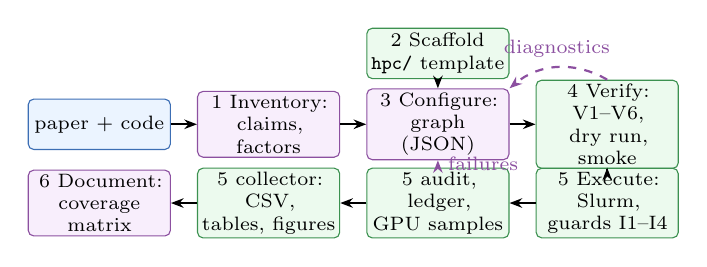
\begin{tikzpicture}[font=\scriptsize,
  box/.style={draw, rounded corners=2pt, align=center, minimum height=6.4mm, text width=17mm, inner sep=1.5pt},
  ag/.style={box, fill=agentbg, draw=agentc},
  pr/.style={box, fill=progbg, draw=progc},
  da/.style={box, fill=databg, draw=datac},
  arr/.style={-{Stealth[length=1.6mm]}, thick}]
\node[da] (in) at (0,0) {paper + code};
\node[ag] (inv) at (2.15,0) {1 Inventory:\\claims, factors};
\node[ag] (cfg) at (4.3,0) {3 Configure:\\graph (JSON)};
\node[pr] (scf) at (4.3,0.9) {2 Scaffold\\\code{hpc/} template};
\node[pr] (ver) at (6.45,0) {4 Verify: V1--V6,\\dry run, smoke};
\node[pr] (run) at (6.45,-1.0) {5 Execute: Slurm,\\guards I1--I4};
\node[pr] (aud) at (4.3,-1.0) {5 audit, ledger,\\GPU samples};
\node[pr] (col) at (2.15,-1.0) {5 collector: CSV,\\tables, figures};
\node[ag] (doc) at (0,-1.0) {6 Document:\\coverage matrix};
\draw[arr] (in) -- (inv); \draw[arr] (inv) -- (cfg); \draw[arr] (scf) -- (cfg);
\draw[arr] (cfg) -- (ver); \draw[arr] (ver) -- (run); \draw[arr] (run) -- (aud);
\draw[arr] (aud) -- (col); \draw[arr] (col) -- (doc);
\draw[arr, dashed, agentc] (ver.north) to[bend right=35] node[above, font=\scriptsize]{diagnostics} (cfg.north east);
\draw[arr, dashed, agentc] (aud.north) -- node[right, font=\scriptsize, pos=0.5]{failures} (cfg.south);
\end{tikzpicture}
\caption{Workflow of \tool{}. Purple: the agent proposes. Green: fixed programs check, run and record. Validator diagnostics and audited failures send the agent back to the graph, never to the checks.}
\label{fig:overview}
\end{figure}

\emph{Running example.} Lena, a PhD student, has a new prompting technique for code generation. She wants to know whether it makes seven open-weight code models (7B to 32B parameters) pass more tests on HumanEval+ (164 tasks) and ClassEval (100 tasks). Her technique plus seven baselines and ablations make eight conditions; with three seeds this gives $8 \times 7 \times 264 \times 3 = 44{,}352$ runs. She has never written a Slurm script. She installs \tool{} (Listing~\ref{lst:use}) and asks Claude Code: ``\textit{Here is my repository and \code{paper.tex}. Run all experiments of the paper on the cluster's GPUs, smoke-test the pipeline first, and give me tables and figures.}'' The agent then runs the commands of Listing~\ref{lst:use}, asking her consent before anything is queued.

\emph{Workflow.} The skill guides the agent through six phases (Fig.~\ref{fig:overview}). The agent (1)~lists the paper's claims, factors and metrics and maps each to the script that produces it, asking Lena whenever paper and code disagree; (2)~copies the template into \code{hpc/}; and (3)~writes the experiment graph as one JSON file (Listing~\ref{lst:graph}). Programs then (4)~verify the graph with a self-test, a dry run and a smoke run, and (5)~execute it, while an audit reports progress and a final \emph{collector} turns raw outputs into tables and figures. Finally, the agent (6)~writes a guide around a coverage matrix from every claim to the steps and files that produce it, for the human to review. This is the key design decision: the agent writes only configuration and a guide, and every check is fixed template code, so a mistake in the graph surfaces as an error message, not as a wrong number.

\begin{lstlisting}[language=json, caption={Lena's experiment graph (\code{hpc/config/experiments.json}). ``\ldots'' elides five models and the \code{run} command is wrapped for print; with both restored, the file passes the self-test. \code{\{RESULTS\}} and \code{\{CELL\}} are set by the runner.}, label=lst:graph, float=t]
{"project": "prompt-study",
 "vars":  {"SEEDS": "1,2,3", "N": "all"},
 "smoke": {"vars": {"SEEDS": "1", "N": "2"}, "matrix_limit": 2},
 "stages": [
  {"name": "setup",
   "resources": {"gpus": "h100:1", "time": "02:00:00"},
   "steps": [
    {"name": "pull", "cmd": "bash pull_models.sh", "critical": true},
    {"name": "preflight", "critical": true,
     "cmd": "python run.py --n 1 --out {RESULTS}/pre.jsonl",
     "produces": ["pre.jsonl"]}]},
  {"name": "generate",
   "depends": [{"stage": "setup", "type": "afterok"}],
   "matrix": {"model": ["qwen2.5-coder-7b", ..., "starcoder2-15b"],
              "bench": ["humaneval_plus", "classeval"]},
   "resources": {"gpus": "h100:1", "time": "24:00:00",
                 "requeue": true},
   "steps": [{"name": "run", "needs": ["pre.jsonl"],
     "cmd": "python run.py --model {model} --bench {bench}
             --seeds {SEEDS} --n {N} --out {RESULTS}/{CELL}.jsonl",
     "produces": ["{CELL}.jsonl"]}]},
  {"name": "analysis",
   "depends": [{"stage": "setup", "type": "afterok"},
               {"stage": "generate", "type": "afterany"}],
   "resources": {"gpus": "h100_1g.10gb:1", "time": "01:00:00"},
   "steps": [{"name": "tables", "cmd": "python tables.py {RESULTS}"},
             {"name": "collect", "builtin": "collect"}]}]}
\end{lstlisting}

\emph{Experiment graph.} Lena's graph (Listing~\ref{lst:graph}) has three \emph{stages}; each becomes one Slurm job or job array whose tasks run an ordered list of \emph{steps} (shell commands). A stage with a \code{matrix} (a parameter grid) becomes a job array with one task per \emph{cell}: here 14 matrix jobs, one per model and benchmark, each loading its model on its own H100 and running its cell's 3{,}936 (HumanEval+) or 2{,}400 (ClassEval) runs. Dependencies have experimental roles. \code{afterok} makes \code{setup} a \emph{gate}: if it fails, Slurm cancels every stage that depends on it with \code{afterok} before it starts (\tool{} passes \code{--kill-on-invalid-dep=yes}). \code{afterany} lets \code{analysis} run on whatever data exists, so one failed cell does not block the study. \code{aftercorr} (unused here) starts cell~$i$ of a stage once cell~$i$ upstream has succeeded. Each step also declares a \emph{data contract}: the files it \code{needs} must exist before it runs and those it \code{produces} must exist after it succeeds, or it fails with a dedicated exit code and a note in the audit. The scheduler orders the jobs; the contracts check that the hand-off happened.

\emph{Checks before submission.} Without running anything, a validator requires unique, file-safe stage names (V1); dependencies only on earlier stages, so no cycle is possible (V2); the same number of cells on both sides of \code{aftercorr} (V3); a GPU or GPU slice for every stage not marked CPU-only (V4); a value for every placeholder such as \code{\{model\}} in every cell of the full and smoke graphs (V5); and a well-formed \code{sbatch} command per stage (V6). \emph{Guards inside jobs.} One shared job script enforces four invariants. It refuses to compute outside a Slurm job, so nothing heavy runs on the login node (I1). It stops if no GPU is visible, and samples GPU utilisation every 60\,s so that an idle GPU becomes visible (I2). It makes reruns safe: finished steps are skipped, and commands that append results skip records already written (I3). For stages marked \code{requeue}, it requeues the job about 15 minutes before its time limit, so long grids continue instead of being cut off (I4).

\emph{Smoke run, audit and results.} The smoke graph keeps every stage, dependency and step but shrinks the work (one seed, two tasks per benchmark, the first two cells of every matrix, short time limits). A passing smoke run has thus executed every stage, step, dependency and data contract at least once on GPU nodes, in minutes, like a test suite with full statement coverage; it does not reach every cell (here, only one of seven models). During a run, the audit (\code{status.sh}) prints one row per stage and cell (state, node, run time against the limit, steps done, records written) and the log lines of every failed step; it refreshes at most once a minute and exits when the queue is empty. The collector exports CSV files, \LaTeX{} tables, figures, the step ledger, GPU usage per job and a manifest (git commit, content hashes, frozen configuration).

\section{Evaluation}\label{sec:eval}

\emph{Setting.} We ran \tool{} on Nibi, a Slurm cluster of the Digital Research Alliance of Canada with up to four H100 80\,GB GPUs per node, many split into MIG slices (isolated GPU shares), under an ordinary allocation. \textbf{RQ1} (benefit): which failures are caught early, how much parallelism is gained, and what the tool reveals that the scheduler's default view does not. \textbf{RQ2} (cost): what do the machinery and its configuration cost? \textbf{RQ3} (reuse): how does the agent fare on published Artifacts? For RQ1--2 we use a \emph{pilot}: a real 44{,}352-run study with Lena's design (14 matrix jobs) plus side studies, 26 jobs and 122 steps on one or two H100s each. Its graph was written by the template's authors, so RQ1--2 test the template and RQ3 the agent. The pilot's coverage matrix maps 32 claims to producing steps and lists the paper's untested aspects as \emph{not covered}. All values come from \code{sacct} records of all 188 jobs of 11 pilot submissions, step ledgers, GPU samples and timings of the released template, or are derived from them.

\begin{figure*}[t]
\centering
\pgfplotsset{every axis/.append style={height=3.75cm, label style={font=\scriptsize}, tick label style={font=\tiny},
  xmajorgrids, ymajorgrids, grid style={black!10}, legend style={font=\tiny, draw=black!20, fill=white, fill opacity=0.85, text opacity=1}, legend cell align=left}}
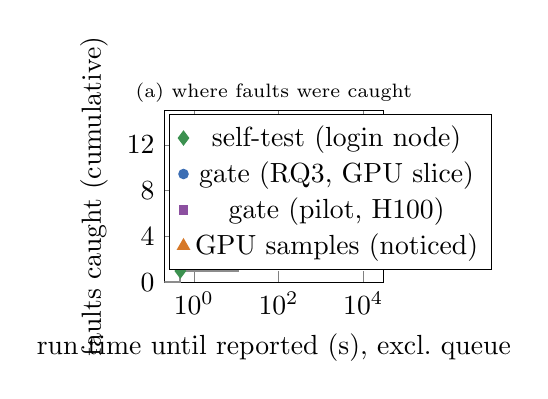
\begin{tikzpicture}
\begin{axis}[width=0.36\textwidth, xmode=log, log basis x=10,
  xlabel={run time until reported (s), excl.\ queue}, ylabel={faults caught (cumulative)},
  xmin=0.2, xmax=30000, ymin=0, ymax=15, ytick={0,4,8,12},
  legend style={at={(0.02,0.98)}, anchor=north west}, title={\scriptsize (a) where faults were caught}, title style={yshift=-1.5ex}]
\addplot[const plot, thick, black!45, forget plot] coordinates {(0.2,0) (0.48,1) (11,2) (12,4) (22,6) (55,7) (57,8) (224,9) (983,10) (1099,11) (2666,12) (9000,14) (30000,14)};
\addplot[only marks, mark=diamond*, mark size=2.5pt, color=progc] coordinates {(0.48,1)};
\addplot[only marks, mark=*, mark size=1.7pt, color=datac] coordinates {(11,2) (12,4) (22,6) (224,9) (1099,11) (2666,12)};
\addplot[only marks, mark=square*, mark size=1.6pt, color=agentc] coordinates {(55,7) (57,8) (983,10)};
\addplot[only marks, mark=triangle*, mark size=2.5pt, color=warnc] coordinates {(9000,14)};
\legend{self-test (login node), {gate (RQ3, GPU slice)}, {gate (pilot, H100)}, GPU samples (noticed)}
\end{axis}
\end{tikzpicture}\hfill
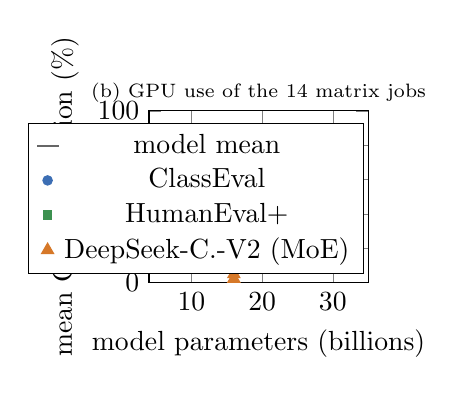
\begin{tikzpicture}
\begin{axis}[width=0.36\textwidth, xlabel={model parameters (billions)},
  ylabel={mean GPU utilisation (\%)}, xmin=4, xmax=35, ymin=0, ymax=100,
  legend style={at={(0.98,0.05)}, anchor=south east}, title={\scriptsize (b) GPU use of the 14 matrix jobs}, title style={yshift=-1.5ex}]
\addplot[only marks, mark=-, mark size=4pt, thick, black!60] coordinates {(7,48.65) (13,67.35) (15,81.4) (20,81.45) (24,76.3) (32,84.5)};
\addplot[only marks, mark=*, mark size=1.7pt, color=datac] coordinates {(7,50.5) (13,58.1) (15,81.6) (20,80.3) (24,75.1) (32,85.0)};
\addplot[only marks, mark=square*, mark size=1.5pt, color=progc] coordinates {(7,46.8) (13,76.6) (15,81.2) (20,82.6) (24,77.5) (32,84.0)};
\addplot[only marks, mark=triangle*, mark size=2.5pt, color=warnc] coordinates {(16,5.0) (16,2.3)};
\legend{model mean, ClassEval, HumanEval+, {DeepSeek-C.-V2 (MoE)}}
\end{axis}
\end{tikzpicture}\hfill
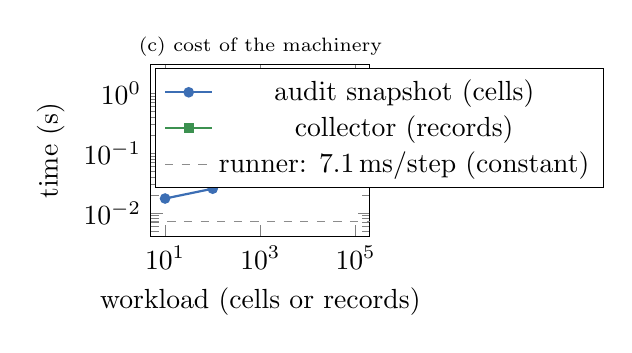
\begin{tikzpicture}
\begin{axis}[width=0.36\textwidth, xmode=log, ymode=log, log basis x=10, log basis y=10,
  xlabel={workload (cells or records)}, ylabel={time (s)}, xmin=5, xmax=200000, ymin=0.004, ymax=3,
  legend style={at={(0.02,0.98)}, anchor=north west}, title={\scriptsize (c) cost of the machinery}, title style={yshift=-1.5ex}]
\addplot[thick, mark=*, mark size=1.5pt, color=datac] coordinates {(10,0.0174) (100,0.0254) (1000,0.1220) (5000,0.5210)};
\addplot[thick, mark=square*, mark size=1.4pt, color=progc] coordinates {(10000,0.17) (100000,1.41)};
\addplot[dashed, black!45, domain=5:200000, samples=2] {0.0071};
\legend{audit snapshot (cells), collector (records), {runner: 7.1\,ms/step (constant)}}
\end{axis}
\end{tikzpicture}
\caption{Benefit and cost, measured on Nibi. (a)~The 14 observed faults (pilot and RQ3) by the run time of the layer that reported them, excluding queue waits: twelve were reported within 45 minutes by the self-test or a setup gate; the two idle GPU jobs were visible in the samples from the start but noticed in a snapshot after 2.5 hours. (b)~Mean GPU utilisation of the full pilot's 14 matrix jobs (159--176 samples of 60\,s each) against total model size; without the two idle DeepSeek-Coder-V2 jobs, it tends to grow with size (Spearman $\rho=0.83$, $n=6$ model means, exact $p=0.06$). (c)~Login-node cost of the audit and the collector.}
\label{fig:eval}
\end{figure*}


\begin{table}[t]
\centering\footnotesize
\caption{Benefit and cost at a glance ($^\dagger$upper bound).}
\label{tab:benefit}
\setlength{\tabcolsep}{3pt}
\begin{tabular}{@{}>{\raggedright\arraybackslash}p{2.2cm} >{\raggedright\arraybackslash}p{3.15cm} >{\raggedright\arraybackslash}p{2.5cm}@{}}
\toprule
Aspect & With \tool{} & Without these checks (worst case) \\
\midrule
\multicolumn{3}{@{}l}{\emph{Benefit (RQ1)}}\\
Failed setup gates & 11 (3 pilot, 8 RQ3); 87/87 dependents cancelled & dependents start \\
GPU cost of one failed pilot setup & 0.02--0.27 GPU-h & $\le$696 GPU-h requested$^\dagger$ \\
Concurrency & makespan 18--24\,min (smoke), 2.0--2.7$\times$; mean 14.6 jobs (full, 3.1\,h) & serial sum: 44--50\,min \\
Silently idle GPU jobs & 2 of 14 exposed (2--5\% util.) & shown as running \\
Faults of our own & 4 of 14 (2 template, 2 agent) & --- \\
\midrule
\multicolumn{3}{@{}l}{\emph{Cost (RQ2, RQ3)}}\\
Machinery & 7.1\,ms/step; audit 0.52\,s at 5{,}000 cells & --- \\
Smoke GPU time & 1.06--1.19 GPU-h per run & --- \\
Configuration & 54--225 lines, 0 edits & hand-written scripts \\
\bottomrule
\end{tabular}
\end{table}

\emph{RQ1, benefit 1: failures are cheap.} Three pilot submissions failed in the setup gate because model downloads broke off (Table~\ref{tab:benefit}). Each time, Slurm cancelled all 25 dependents (14 matrix jobs and 11 side-study and analysis jobs) before allocation: 75 jobs, none of which used a GPU-second. Each failure cost 0.02--0.27 GPU-hours. Without the gate, the dependents' requested resources (29 H100s for at most 24 hours) bound the exposure at 696 GPU-hours per submission; most would have crashed early, but nothing would have stopped them from starting or writing partial outputs. Fig.~\ref{fig:eval}a places all 14 faults we observed on the run time of the layer that reported them. Twelve were caught by the cheapest layers: a template defect by the self-test in 0.5\,s, and eleven by setup gates within 11\,s to 44\,min. Four were self-inflicted (two template defects, two agent errors), all caught before any main job. The last two faults were idle GPU jobs, visible in the samples from the start but noticed after 2.5 hours.

\emph{Benefit 2: Slurm parallelism by default.} All stages are queued at once and Slurm resolves their dependencies, so independent jobs run side by side and queue waits overlap with computation. Each smoke run (10 jobs, 36 steps) used 7--8 nodes; its makespan (first job start to last job end) was 18--24 minutes against 44--50 minutes of summed job time, a concurrency of 2.0--2.7$\times$ (2.68, 2.05, 2.39). The makespan is bounded below by a 16-minute critical path, and the ratio is conservative, because serial execution would also queue before each job. In a snapshot of the full run after 3.1 hours, 19 of 26 jobs had started, on average 14.6 at a time, with no failed step. This parallelism is Slurm's; \tool{} makes a novice's graph expose it.

\emph{Benefit 3: hidden problems.} In \code{squeue} and default \code{sacct} fields, all 14 matrix jobs looked healthy. The GPU samples of guard I2 told another story (Fig.~\ref{fig:eval}b). Twelve jobs averaged 73\% utilisation, but the two DeepSeek-Coder-V2 jobs had used their GPUs at 2--5\% for over 2.5 hours. They were not failing, so no other signal would have flagged them. The cause is not yet diagnosed; possibly relevant, the model is a mixture of experts with about 2.4B active parameters. Across the other six models, utilisation tends to grow with size (Spearman $\rho = 0.83$ over $n = 6$ model means, exact $p = 0.06$; $\rho = 0.75$ over the 12 jobs), from 47--51\% at 7B to 84--85\% at 32B. One unmeasured hypothesis is that small models leave the GPU waiting while the CPU runs the tests.

\emph{RQ2: cost.} The machinery is cheap (Fig.~\ref{fig:eval}c; medians on the login node). Scaffolding takes 0.18\,s and the self-test 0.48\,s. The in-job step runner adds 7.1\,ms per executed step and 1.2\,ms per skipped one. An audit snapshot takes 17\,ms for 10 cells and 0.52\,s for 5{,}000 (about 0.1\,ms per additional cell); collecting 100{,}000 records takes 1.4\,s. The real cost is the smoke run's GPU time: 1.06--1.19 GPU-hours per pilot smoke run, 2.0--2.3\% of what the full run had used in its first 3.1 hours (51.8 GPU-hours). We did not measure the agent's own cost (session time, tokens) or human interventions.

\subsection{RQ3: Ten Unseen Artifacts}\label{sec:study}

\emph{Selection.} We mined all 4{,}814 publications of 2024--2026 by ICSE, FSE, ASE, TSE, EMSE and TOSEM from OpenAlex~\cite{priem2022openalex} (4{,}187 of them research papers). Scripted filters kept papers on LLMs (1{,}574); those linking a GitHub Artifact in their full text (584 papers, 569 repositories); and repositories that clone (474), use open-weight models (310) and are Python projects with dependencies and run commands (118). We screened these by a fixed score (favouring local model serving, documented commands and recent activity) until ten met all of: open-weight models of at most 34B parameters, public data, no Docker (unavailable on the cluster), at most an estimated 300 H100-hours (24 decisions, one reversed after cloning). For each Artifact, a new Claude Code session with \tool{} read the paper and repository and wrote the configuration: a \emph{full} rerun for six, and for the four where it reported blocking defects in the documented commands, \emph{probes} that run each README step once at minimal size, so an exit code can confirm the defect.



\begin{table}[t]
\centering\scriptsize
\caption{RQ3 Artifacts: gates in submission order (\xmark{} failed, \cmark{} passed, --- withdrawn), configuration lines (+ glue), H100-equivalent hours.}
\label{tab:study}
\setlength{\tabcolsep}{1.9pt}
\begin{tabular}{@{}l l l r c l r@{}}
\toprule
Artifact & Venue & Mode & Config. & Gates & Failures & H100-h \\
\midrule
SemGuard~\cite{wang2025semguard} & ASE'25 & probe & 149 & --- & & --- \\
ProvenanceGuard~\cite{she2026provenanceguard} & ASE'26 & full & 162 & \xmark\cmark & wheel & 0.007 \\
RetriGen~\cite{zhang2025retrigen} & TOSEM'25 & full & 130+42 & \xmark\xmark & wheel, agent & 0.046 \\
ExeCRE~\cite{dong2026execre} & ASE'26 & full & 225+18 & \xmark\xmark\cmark & wheel, data & 0.024 \\
EffiSkel~\cite{yu2026effiskel} & FSE'26 & probe & 161 & --- & & --- \\
BinarySPD~\cite{li2026binaryspd} & TOSEM'26 & full & 164 & \xmark\cmark & wheel & 0.005 \\
IRCoCo~\cite{li2024ircoco} & FSE'24 & probe & 149 & --- & & --- \\
RobustExt~\cite{rabbi2026robustness} & EMSE'26 & full & 116+45 & \cmark & & 0.004 \\
LLM4Perf~\cite{wang2026llm4perf} & ICSE'26 & full & 54 & \xmark\xmark & templ., agent & 0.108 \\
LogReasoner~\cite{ma2026logreasoner} & TOSEM'26 & probe & 137 & --- & & --- \\
\midrule
Total & \multicolumn{2}{l}{6 full, 4 probe} & 1{,}552 & 8\xmark\,4\cmark & & 0.19 \\
\bottomrule
\end{tabular}
\end{table}

\emph{Results.} Table~\ref{tab:study} covers the first round: the setup gates of the six full Artifacts' smoke runs (the probes never ran). The ten graphs have 32 stages and 97 steps, in 54--225 lines of configuration each (graph, comparison script, model-server hooks); three also needed 18--45 lines of glue between documented steps, and none needed an edit. Including resubmissions, 12 gates ran and 8 failed: four on wheel resolution against the cluster's curated package store (its \emph{wheelhouse}: one pin without a build, one missing package, two OpenCV wheels provided only as a module), one on a dataset loader that asks an interactive question in a batch job, two on the agent's configuration (a pipeline exiting with SIGPIPE, a script expecting a missing column), and one on our template. Slurm cancelled all 12 dependents of the failed gates before allocation; fixes were resubmitted after a median of 8.3 minutes (3--13, $n = 6$). The round cost 0.19 H100-equivalent hours; four full Artifacts passed their gate. All queued jobs, including the four probes, were then withdrawn before any main stage started, so reproduction accuracy remains open. Configuration alone exposed Artifact gaps: suspected defects, not yet confirmed by execution, in all four probe Artifacts; missing steps in three full Artifacts; and one Artifact without evaluation code, whose comparison step reports \emph{not comparable} instead of silently passing.

\section{Related Work}\label{sec:related}

\emph{Workflow systems} such as Pegasus~\cite{deelman2015pegasus}, Snakemake~\cite{molder2021snakemake}, Nextflow~\cite{ditommaso2017nextflow} and Parsl~\cite{babuji2019parsl} describe computations as task graphs for schedulers, with file dependencies much like our data contracts. They are mature and general, but describe \emph{how} to compute, not \emph{which claims} a result supports, and need their own language and engine; \tool{} uses one checkable JSON graph and plain Slurm arrays and dependencies, and a step can still call such a workflow. \emph{Reproducibility aids} such as ReproZip~\cite{chirigati2016reprozip}, the Popper convention~\cite{jimenez2017popper}, Artifact-sharing practices~\cite{timperley2021artifact} and LLM-study guidelines~\cite{baltes2025guidelines} make computations rerunnable; \tool{} adds an agent that derives the pipeline from a paper's claims. Like Boa~\cite{dyer2013boa} for ultra-large-scale mining, \tool{} makes a costly MSR workflow accessible. \emph{Agents for research}, benchmarked by SUPER~\cite{bogin2024super}, CORE-Bench~\cite{siegel2024corebench} and PaperBench~\cite{starace2025paperbench}, set up repositories or replicate papers, typically in one container; separately, LLMs now write parallel HPC code~\cite{nichols2024hpccoder}. These works measure what an agent \emph{can} do; \tool{} constrains and checks what it \emph{may} do on a shared cluster.

\section{Limitations, Future Work and Conclusion}\label{sec:concl}

\emph{Limitations.} \tool{} needs Claude Code to write the configuration, though the generated pipeline runs without it; the agent is instructed, not forced, to leave the template unchanged, and its claim mapping is reviewed by the human, not checked by code. Other Slurm sites would need changes to \code{cluster.env}, the GPU names and possibly the wheelhouse set-up; we have tested none. MIG slices report no utilisation to \code{nvidia-smi}, so I2 cannot sample them (the pilot's matrix jobs used whole GPUs). Our evidence comes from one cluster; the pilot's full run is a 3.1-hour snapshot, so I4 was not exercised; and the RQ3 Artifacts were executed only up to their gates. The data thus show cheap, early fault detection, not yet faithful reproduction. A wrong metric runs as smoothly as a right one, so where Artifacts ship raw outputs, the RQ3 configurations first re-score them, to separate metric code from rerun.

\emph{Future work and conclusion.} We will finish the ten-Artifact reruns under tolerances fixed in advance, check cheaply before expensive downloads, and support other schedulers. AI has made writing software cheap; \tool{} aims to make checking it at scale cheap as well.

\smallskip\noindent\textbf{Availability.}\label{sec:data} \tool{} is open source at \url{https://github.com/ai4se4ai-lab/use-hpc-claude-skill}; its self-test runs without Slurm. A release with the running example, pilot ledgers and RQ3 configurations will be archived on Zenodo.
% TODO(author): insert the Zenodo DOI and confirm the licence file in the repository.

\bibliographystyle{IEEEtran}
\bibliography{references}

\end{document}